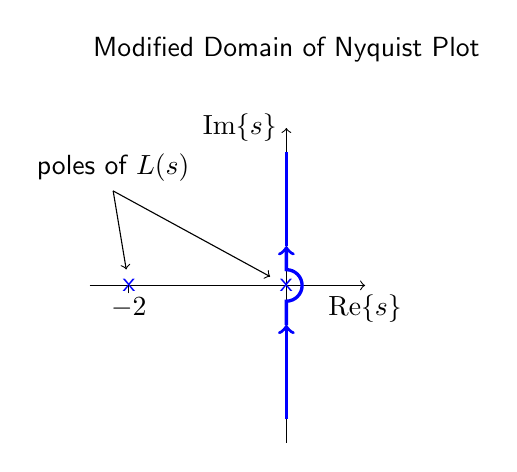
\begin{tikzpicture}[
sysblock/.style={draw,rectangle,inner sep=6pt,minimum width=1.25cm,minimum height=1.0cm,very thick},
summer/.style={circle,draw,very thick}]
\draw (-4,3) node {\textsf{Modified Domain of Nyquist Plot}};
\draw[->] (-4,-2) -- ++(0,4) node[left] {Im$\{s\}$};
\draw[->] (-6.5,0) -- ++(3.5,0) node[below] {Re$\{s\}$};
\draw[->,very thick,color=blue] (-4,-1.7)  -- (-4,-.5); 
\draw[->,very thick,color=blue] (-4,-.5) -- (-4,-0.2) arc (-90:90:.2) -- (-4,.5); 
\draw[very thick,color=blue] (-4,.5) --  (-4,1.7);
\draw (-4,0) node (po1) {\color{blue}\textsf{x}};
\draw (-6,0) node (po2) {\color{blue}\textsf{x}};
\draw (-6,-.1) node[below=-2pt] {$-2$} -- ++(0,.1);
\draw (-6.2,1.5) node (text) {\textsf{poles of $L(s)$}};
\draw[->] (text.-90) -- (po1);
\draw[->] (text.-90) -- (po2);


\end{tikzpicture}